\chapter{Introduction}


% Description of large-scale structure in our universe
%  - What has been observed?
%  - What has been simulated?

\begin{figure}
    \includegraphics[width=0.65\textwidth]{Images/Intro/sdss}
    \caption[SDSS galaxy map]{A slice through the SDSS galaxy 
    distribution\footnote{\url{http://www.sdss.org/science/orangepie/}}; each 
    point on this plot is a galaxy.  Large sky surveys such as SDSS have 
    revealed a non-uniform distribution of galaxies throughout the universe.  
    Dubbed the cosmic web, galaxies clump together in clusters and along 
    filaments, leaving giant gaps between them (similar to a sponge).}
    \label{fig:SDSS_map}
\end{figure}

\begin{figure}
    \includegraphics[width=0.9\textwidth]{Images/Intro/Millenium_simulation}
    \caption[Dark matter simulation]{Snapshots of a portion of the Millenium 
    Simulation\footnote{\url{https://wwwmpa.mpa-garching.mpg.de/galform/virgo/millennium/}} 
    showing the dark matter distribution at different points in time from 0.21 
    Gyr after the Big Bang to the present.  Small perturbations in the initial 
    distribution of dark matter are amplified as the universe expands.  Gravity 
    causes the slightly overdense regions to contract while simultaneously 
    causing the underdense regions to expand.}
    \label{fig:DMsim}
\end{figure}

Large galaxy surveys such as the Sloan Digital Sky Survey \citep[SDSS;][]
{York00} have revealed a non-uniform distribution of galaxies throughout 
the universe.  Taking on a shape similar to that of a sponge-like topology 
\citep{Gott98} or a three-dimensional cosmic web \citep{Bond96}, galaxies clump 
together in clusters and along filaments, leaving void regions between these 
large-scale structures.  Evidence of this distribution can be seen in Fig. 
\ref{fig:SDSS_map} for galaxies in the SDSS Data Release 7 \citep[SDSS DR7;][]
{Abazajian09}.  Based on these observations, dark matter simulations have been 
constructed which successfully reproduce the same large-scale structure.  If we 
start with a mostly uniform distribution of dark matter at the Big Bang with 
quantum mechanical perturbations, Fig. \ref{fig:DMsim} outlines the evolution of 
that dark matter up through the present.  These snapshots from the Millenium 
Simulation project \citep{Springel05} show that small perturbations in the 
initial distribution of dark matter are amplified as the universe expands.  
Gravity causes the slightly overdense regions to collapse while simultaneously 
causing the underdense regions to expand.  Due to dark matter's gravitational 
attraction, we believe that the baryonic mattter (matter which interacts 
electromagnetically) will trace the dark matter distribution, resulting in the 
galaxy distribution we observe today.


% Void galaxies
\begin{figure}
    \includegraphics[width=0.9\textwidth]{Images/Intro/VoidFinder}
    \caption[Sky map highlighting voids and void galaxies]{A 10 \hMpc slice of 
    SDSS DR7 \citep[Fig. 1]{Moorman14} with void regions highlighted in blue 
    circles.  Void galaxies are shown as red points while wall galaxies are 
    black.  Existing in the cosmological voids (space between the galactic 
    filaments), void galaxies are though to demonstrate the fundamental 
    characteristics of galactic evolution.}
\end{figure}

Existing in the cosmological voids, void galaxies are thought to demonstrate the 
fundamental characteristics of galactic evolution.  Cosmic voids are an 
important environment for studying galaxy formation \citep[see][for a review]
{vandeWeygaert11}.  Gravitational clustering proceeds as if in a very low 
density universe, where the amassment of gravitationally bound dark matter halos 
ends relatively early and there is little subsequent interaction between the 
galaxies due to the lower density and the faster local Hubble expansion.  
Therefore, $\Lambda$CDM cosmology predicts that galaxies formed in voids should 
have lower mass and be retarded in their star formation when compared to those 
in denser regions \cite[e.g.,][]{Gottlober03,Goldberg05,Cen11}.  
\cite{Goldberg04} show that a void region that is only 10\% of the mean density 
of the universe with $\Omega_{matter} = 0.3$, $h = 0.7$ dynamically evolves as 
if $\Omega_{matter} = 0.02$, $\Omega_\Lambda = 0.48$, and $h = 0.84$.  
Additionally, hydrodynamical cosmological simulations by \cite{Cen11} show that 
void galaxies may continue to form stars because the gas in voids remains below 
the critical entropy threshold (above which the cooling time exceeds the Hubble 
time).  Void galaxies evolve in a relatively pristine environment where 
interactions are rare and star formation proceeds up to the present epoch 
because void galaxies are able to retain their gas.  This contrasts with denser 
environments, where the chemical composition and evolution of galaxies are 
drastically altered due to mergers and tidal and/or ram-pressure stripping.

% What do we already know about the environmental influence?
Observational studies of void galaxies have included investigation of 
photometric properties such as luminosity \citep{Hoyle05,Croton05,Moorman15}, 
color and morphological type \citep{Grogin00,Rojas04,Patiri06,Park07,
vonBendaBeckmann08,Hoyle12}, star formation rates estimated from optical 
spectroscopy and UV photometry \citep{Rojas05,Moorman15,Beygu16}, and gas 
content \citep{Kreckel12,Moorman16,Jones16}.  When compared to galaxies in 
denser regions, void galaxies tend to be fainter, of late morphological types, 
bluer, forming stars at higher rates per unit stellar mass, and more gas rich.

% Dwarf galaxies
\begin{figure}
    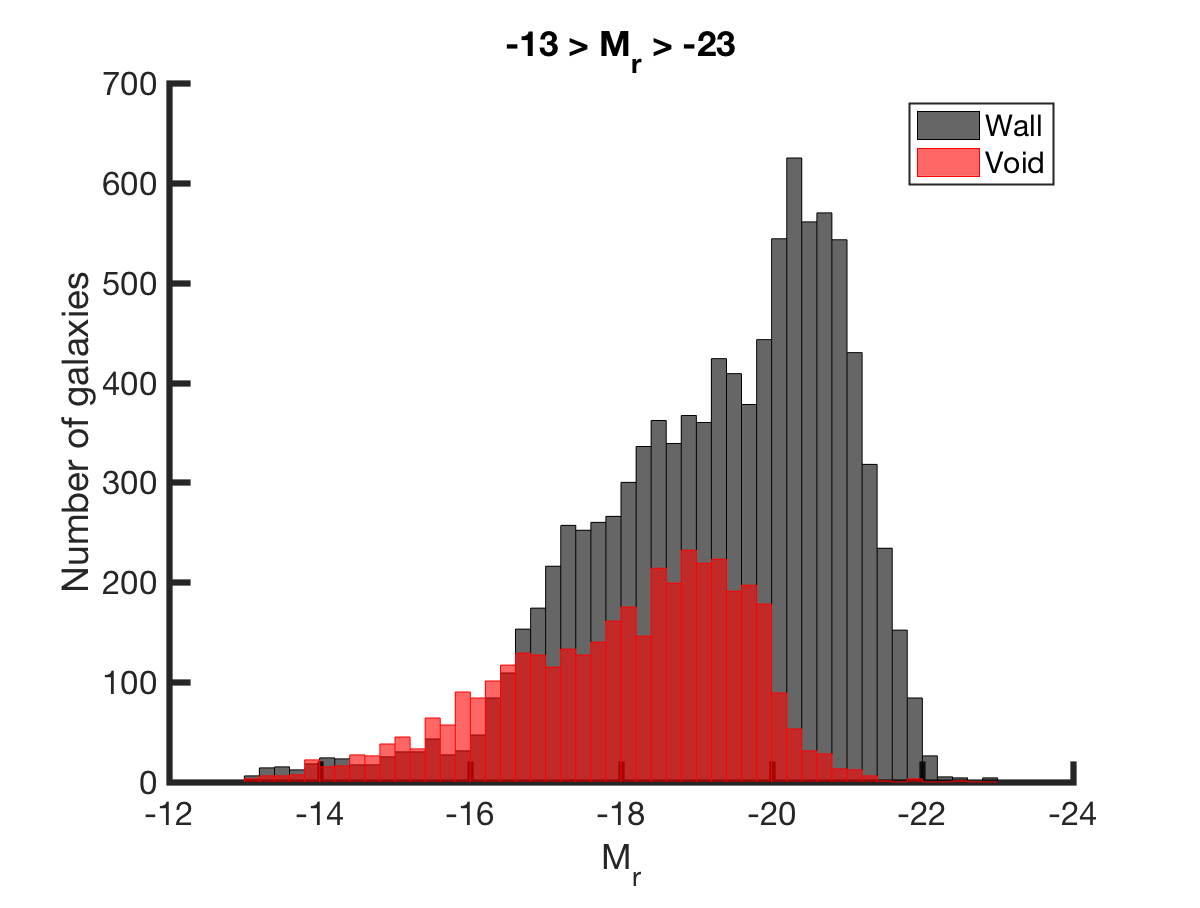
\includegraphics[width=0.65\textwidth]{Images/Intro/1sig_13-23_SDSS_Mr_hist_count_fill}
    \caption[Absolute magnitude distribution of galaxies in SDSS DR7]{Absolute 
    magnitude ($M_r$) distribution of galaxies in SDSS DR7, separated into void 
    and wall environments.  Dwarf galaxies are defined as galaxies with absolute 
    magnitudes fainter than -17 ($M_r > -17$).  For reference, the Milky Way has 
    an absolute magnitude $M_r \approx -20$.}
    \label{fig:Mr_SDSS}
\end{figure}

In particular, we study the effects of the large-scale environment on the 
formation and evolution of dwarf galaxies.  Fig. \ref{fig:Mr_SDSS} shows the 
distribution of galaxies by their absolute magnitudes detected in SDSS DR7.  
Defined to be galaxies with absolute magnitudes fainter than -17 ($M_r > -17$), 
the low stellar masses of dwarf galaxies correspond to more shallow 
gravitational potential wells.  This causes any environmental effects to have a 
more significant influence on dwarf galaxies than on galaxies with larger 
stellar masses.  In addition, studying void dwarf galaxies will complement 
previous studies of dwarfs in groups and clusters because the assembly histories 
of low-mass galaxies are predicted to be very different \citep[e.g.,][]{Gao07,
Lackner12}.  Observations to date also show that the properties of dwarf 
galaxies vary dramatically with the environment \citep[e.g.,][]{Ann08,Geha12}.



% Metallicity
%  - How are elements synthesized in stars?
%  - What does the light look like when it reaches us?  When we look at an emission spectrum, what are we studying?
%  - What are forbidden transitions and why are they important?
%  - How do we get the temperature from the emission line ratio?  (Summary - refer to appendix for more details)
%  - What is the metallicity?  O/H - Why oxygen?  and once we estimate the abundances of each ion, we add them together to get the total abundance for that element

The first stars that formed are thought to have been composed of hydrogen and 
helium (and trace amounts of other primordial elements).  As stars burn, 
nucleosythesis creates heavier elements at the core.  When the stars expel their 
contents in supernovae and stellar winds, the heavier elements are distributed 
between the surrounding interstellar gas and circumgalactic medium.  By 
measuring the ratio of elements heavier than helium (``metals'') relative to the 
hydrogen content, we measure the integrated star formation history of the 
galaxy.  This ``metallicity'' is commonly expressed as \OH, although it is 
sometimes given in units of the solar metallicity, $Z/Z_\odot$.

\begin{figure}
    \includegraphics[width=0.9\textwidth]{Images/Intro/Kirchoff}
    \caption[Kirchoff's laws of spectroscopy]{Three different viewpoints of the 
    light emitted from a star and/or a cool cloud of gas, representing 
    Kirchoff's laws of 
    spectroscopy\footnote{\url{http://courses.atlas.illinois.edu/spring2011/astr/astr210/LECTURES/Lect12.html}}.  
    A star emits light across all wavelengths, so the resulting spectrum is 
    known as a continuous spectrum.  Star's light that has passed through a 
    cloud of cool gas before being observed is an absorption spectrum, where the 
    elements in the cloud have absorbed some of the light at specific 
    wavelengths (corresponding to the particular elements present in the gas).  
    If observed off the line-of-sight of the star, the light emitted from the 
    cloud of cooler gas results in an emission spectrum, where the gas is 
    re-radiating the light it absorbed from the star.}
    \label{fig:Kirchoff}
\end{figure}

We use a galaxy's spectrum to measure various properties of the stellar 
population and interstellar medium.  A galaxy's spectrum is a superposition of 
light from the stars and emission lines from the interstellar gas.  The 
observer's viewpoint determines the type of spectrum measured.  As shown in Fig. 
\ref{fig:Kirchoff}, if we separate a star's light by its wavelength, we will 
observe a continuous spectrum, since its photosphere is close to a blackbody.  
If instead we observe the starlight after it has passed through a cloud of 
cooler gas (relative to the temperature of the star), we will measure an 
absorption line spectrum; the elements in the gas cloud have absorbed some of 
the star's light at specific wavelengths corresponding to the particular ions 
present.  Finally, if we only observe the light emitted from the cool gas cloud, 
we will measure an emission line spectrum.  The method we employ to estimate the 
metallicity of a galaxy requires the detection of particular emission lines.  We 
study the gas-phase chemical abundances of \ion{H}{2} regions in a galaxy, where 
the light is coming from low-density gas partially ionized by UV photons emitted 
from young, hot stars.  Therefore, we are measuring the abundances of the 
elements produced in previous generations of stars.

\begin{figure}
    \includegraphics[width=0.9\textwidth]{Images/Intro/spectrum}
    \caption[Sample (void) dwarf galaxy spectrum]{Example SDSS DR7 
    spectrum\footnote{\url{http://cas.sdss.org/dr7/en/get/specById.asp?ID=124634771904004096}} 
    --- this is a void dwarf galaxy whose gas-phase chemical abundances are 
    slightly above average.  The [\ion{O}{3}] $\lambda$4363 auroral line is 
    circled in red, while the [\ion{O}{3}] $\lambda \lambda$4959,5007 doublet is 
    circled in yellow.}
    \label{fig:spectrum}
\end{figure}

The ion transitions observed in the optical part of the spectrum (where SDSS DR7 
operates) consist of forbidden transitions.  As explained in detail in Section 
\ref{sec:physics}, forbidden transitions have much longer lifetimes than the 
allowed electric dipole electron transitions.  These transitions strongly depend 
on the temperature and density of the electron gas, because the long lifetimes 
allow the atoms to easily collisionally de-excite.  By taking the ratio of the 
[\ion{O}{3}] $\lambda$4363 auroral line to the [\ion{O}{3}] 
$\lambda \lambda$4959,5007 doublet, we can get an estimate of the temperature of 
the gas.  These lines are highlighted on the example SDSS DR7 spectrum shown in 
Fig. \ref{fig:spectrum}.  

Oxygen is used as a proxy to measure the metallicity of an \ion{H}{2} region, 
because oxygen is the most abundant element in the universe after hydrogen and 
helium \citep{Emsley11}.  It also has strong emission lines in the visible 
wavelength range, so it is relatively easy to observe.  Oxygen emission is the 
most effective cooling source in an \ion{H}{2} region, so lower metallicities 
correspond to higher temperatures.  There are three main factors which determine 
the strength of an emission line: the gas temperature, the electron density, and 
the relative number of ions in the gas.  It is possible to calculate the number 
ratios for any of the heavy elements with respect to hydrogen once the electron 
temperature and density of the interstellar gas are estimated.


% Outline of Thesis
% Pose the problem - how does the large-scale environment affect galaxy evolution?
We want to understand how the cosmic environment affects the evolution of a 
galaxy and what influence it has on a galaxy's star formation.  To do this, we 
compare the properties of galaxies living in voids with galaxies in denser 
regions in an effort to understand how the properties of the gas and the history 
of star formation in a galaxy depend on the environment.  We then try to infer 
what these results tell us about the dark matter structure and history of the 
galaxy.  In Chapter \ref{ch:Paper1}, we calculate and compare the metallicity of 
135 star-forming dwarf galaxies as a function of their large-scale environment.  
We continue studying this galaxy sample in Chapter \ref{ch:Paper2} by estimating 
their ratios of nitrogen to oxygen and looking at how that depends on the 
large-scale environment.  To expand our dwarf galaxy sample, we derive an 
approximation for the amount of singly-ionized oxygen and repeat our analysis of 
the large-scale environmental influence on the gas-phase chemical abundances of 
1920 star-forming dwarf galaxies in Chapter \ref{ch:Paper3}.  In Chapter 
\ref{ch:smallScaleEnvironment}, we investigate how the dwarf galaxies' 
properties depend on the galaxies' distances to the nearest neighbors and 
groups.  Finally, in an effort to better understand how galaxies evolve from 
blue, star-forming systems to ``red and dead,'' we discover a way to classify 
galaxies into their location on the color-magnitude diagram in Chapter 
\ref{ch:GV}.  We present our conclusions and suggestions for future research in 
Chapter \ref{ch:conclusion}.